% A rounded node whose centred lines TeX may break more than one way: its
% height is a range, and the corners run pgfmath on it.
\documentclass{article}
\usepackage{tikz}
\begin{document}
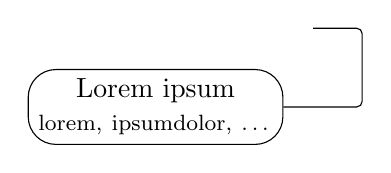
\begin{tikzpicture}
\node[draw,rounded corners=10pt,text width=3cm,align=center] (p) at (0,0) {%
   Lorem ipsum\\
   {\footnotesize lorem, ipsumdolor,~\ldots}
};
\draw[rounded corners=2pt] (p.east) -- ++(1,0) |- (2,1);
\end{tikzpicture}
\gdef\SatexReachedEnd{}
\end{document}
